\section{Movimiento Ondulatorio}

Antes de comenzar con el movimiento ondulatorio te recomiendo que revises el resumen de movimiento armónico simple en la sección \ref{sec:mas}. El movimiento ondulatorio está estrechamente relacionado con el movimiento armónico simple.

Un movimiento ondulatorio es un movimiento que se caracteriza por la transferencia de energía a través del espacio sin el acompañamiento de transferencia de materia. Todas las ondas mecánicas requieren:
\begin{enumerate}
  \item alguna fuente de perturbación
  \item un medio que contenga elementos que puedan ser perturbados y
  \item algún mecanismo físico a partir del cual los elementos del medio puedan influirse mutuamente.
\end{enumerate}

\begin{wrapfigure}{r}{0.3\textwidth}
  \centering
  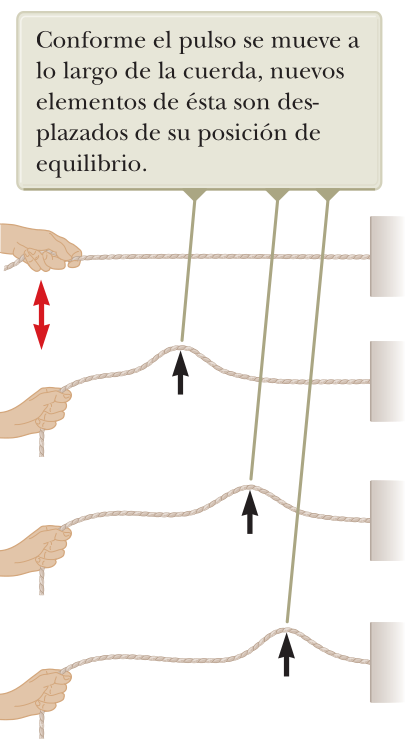
\includegraphics[width=\linewidth]{wave_example.png}
  \caption{Un pulso que viaja a lo largo de la cuerda.}
  \label{fig:wave_example}
\end{wrapfigure}
La onda \textbf{es una perturbación} que experimenta el sistema y que lo aparta de su posición de equilibrio. Una \textit{onda} es un tren de pulsos, es decir, muchos pulsos periódicos (o bien, pulsos iguales seguidos separados uniformemente entre sí).

Por ejemplo, si se observa la figura \ref{fig:wave_example}, una mano mueve una vez, hacia arriba y hacia abajo, el extremo de una cuerda estirada, generando un \textit{pulso} que viaja a lo largo de la cuerda con una rapidez definida. La mano en este caso se denomina \textbf{foco de onda} que es el punto o región desde la cual se origina o se concentra la propagación de la onda.

Lo que se transmite a través de la cuerda, a cada punto cercano, es \textbf{energía, no materia}. Es decir, las partículas que conforman la cuerda no se desplazan a la derecha, sino más bien, se mueven hacia arriba y hacia abajo, y lo que se desplaza a la derecha es el pulso. Las ondas formadas por este tipo de pulso, donde el movimiento de las partículas es \hl{\textit{perpendicular}} a la dirección de propagación del pulso se denominan \textbf{ondas transversales}.

Hay otro tipo de propagación de onda. Aquella onda cuya propagación es \hl{\textit{paralela}} a la perturbación provocada por el pulso se denomina \textbf{onda longitudinal}. Se puede comparar el pulso de onda \textbf{transversal} de la figura \ref{fig:wave_example} con el pulso de onda \textbf{longitudinal} de la figura \ref{fig:longitudinal_wave}.

\begin{figure}[ht]
  \centering
  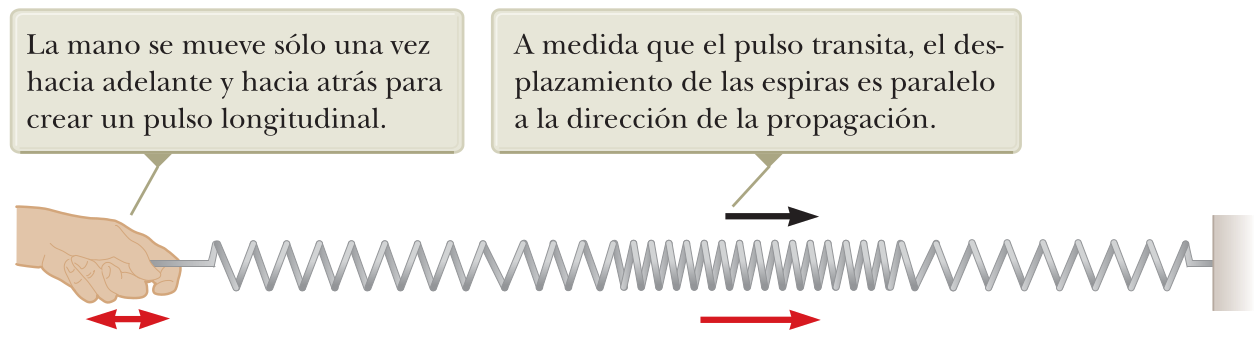
\includegraphics[width=0.8\textwidth]{logitudinal_wave.png}
  \caption{Un pulso que viaja a lo largo de un resorte.}
  \label{fig:longitudinal_wave}
\end{figure}

Para poder poner en movimiento estos medios en los que se propagan las ondas hay que \hl{aportar energía} al sistema realizando trabajo mecánico sobre el mismo. La onda es el transporte de energía de una región del medio a otra. Esa energía cuando llega a cualquier punto del medio, lo aparta de su posición de equilibrio, poniéndolo a vibrar. 

\subsection{Análisis de modelo de onda}

Si tomamos el ejemplo de la cuerda, pero ahora en vez de generar un pulso generamos un tren de pulsos como se muestra en la figura \ref{fig:wave_train} sabemos que la onda será transversal y también que las partículas que conforman la cuerda vibran con un movimiento armónico simple. De ahí podemos definir algunas cantidades importantes.

\begin{figure}[ht]
  \centering
  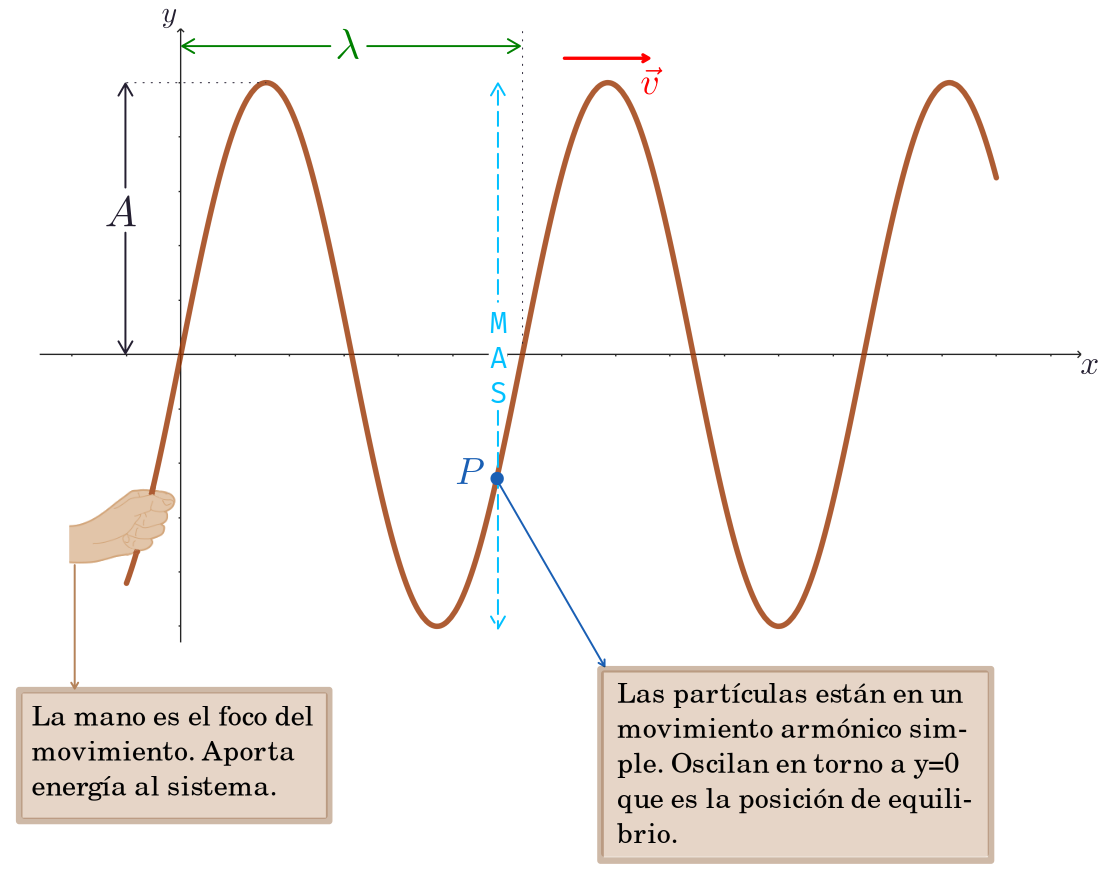
\includegraphics[width=0.8\textwidth]{wave_train.png}
  \caption{Un tren de pulsos que viajan a lo largo de la cuerda.}
  \label{fig:wave_train}
\end{figure}

A continuación te presento las \textit{cantidades físicas básicas} que caracterizan a una onda armónica, junto con su definición, unidad en el SI y su relación con otras magnitudes.

\subsubsection{Cantidades físicas básicas de una onda}
\label{sec:waves_basic_quantities}

\paragraph{Amplitud (\(A\))}

Es el valor máximo que alcanza la magnitud oscilante respecto de su posición de equilibrio.

\begin{itemize}
  \item Unidad: depende del tipo de onda, en el caso de ondas mecánicas su unidad es metros (\(\si{\meter}\)).
  \item Interpretación: indica la intensidad o energía de la onda.
  \item No afecta la velocidad, pero sí la energía transportada.
\end{itemize}

\paragraph{Período (\(T\))}

Es el tiempo que tarda un punto del medio en realizar una oscilación completa. Si vemos la figura \ref{fig:wave_train} el punto \(P\) está en un movimiento armónico simple. Una oscilación completa demora \(T\) segundos, que es un período. 

\begin{itemize}
  \item Unidad: segundos (s).
  \item Relación: inversamente proporcional a la frecuencia: \(T = \frac{1}{f}\)
\end{itemize}

\paragraph{Frecuencia (\(f\))}

Es el número de oscilaciones completas por unidad de tiempo.

\begin{itemize}
  \item Unidad: hertz (Hz), donde \(1\, \text{Hz} = 1\, \text{oscilación/s}\).
  \item Relación: \(f = \frac{1}{T}\)
\end{itemize}

\paragraph{Longitud de onda (\(\lambda\))}

Es la distancia entre dos puntos consecutivos que están en la misma fase (por ejemplo, dos crestas sucesivas). Como se ve en la figura \ref{fig:wave_train} la longitud de onda es la distancia entre dos puntos en fase. 

En una onda mecánica, dos puntos están en fase cuando cumplen las siguientes condiciones:

\begin{enumerate}
  \item Tienen el mismo estado de vibración en el mismo instante, es decir:
    \begin{itemize}
      \item Mismo desplazamiento (posición) respecto a la posición de equilibrio.
      \item Misma velocidad (moviéndose en la misma dirección).
      \item Misma aceleración.
    \end{itemize}
  \item La diferencia de fase entre ellos es un múltiplo entero de \(2\pi\) radianes (o \(0\), \(\pm 2\pi\), \(\pm 4\pi\), etc.). 
  \item La distancia entre ellos es un múltiplo entero de la longitud de onda (\(\lambda\)):
   \[
   \Delta x = n\lambda \quad \text{(con \(n = 0, \pm 1, \pm 2, \dots\))}
   \]
\end{enumerate}

Si la diferencia de fase es \(\pi\) radianes (o un múltiplo impar de \(\pi\)), los puntos están en \textbf{oposición de fase} (máximo alejamiento en vibración). Dos puntos están en fase cuando su separación espacial es un múltiplo entero de \(\lambda\) y su diferencia de fase es \(2\pi n\). Esto implica que oscilan sincronizados.

\begin{itemize}
  \item Unidad: metros (m).
  \item Relación: \(\lambda = \frac{v}{f} = v T\)
\end{itemize}

\paragraph{Velocidad de propagación (\(v\))}

Es la velocidad con que se desplaza el frente de onda (es decir, cómo se propaga la perturbación en el medio).

\begin{itemize}
  \item Unidad: metros por segundo (m/s).
  \item Relación fundamental: la velocidad de propagación de una onda es \(v = \lambda f\)
\end{itemize}

\paragraph{Número de onda (\(k\))}

Es una medida del número de ciclos por unidad de longitud, análogo espacial de la frecuencia temporal.

\begin{itemize}
  \item Unidad: radianes por metro (rad/m).
  \item Relación: \(k = \frac{2\pi}{\lambda}\)
\end{itemize}

\paragraph{Frecuencia angular (\(\omega\))}

Es la frecuencia expresada en términos angulares (radianes por segundo).

\begin{itemize}
  \item Unidad: rad/s.
  \item Relación: \(\omega = 2\pi f = \frac{2\pi}{T}\)
\end{itemize}

\paragraph{Fase (\(\varphi\)) y diferencia de fase}

La fase indica en qué punto del ciclo se encuentra la oscilación. Es el mismo concepto de fase que se encuentra en el movimiento armónico simple. Si no lo recuerdas te recomiendo que revises el capítulo \ref{sec:mas}.

\begin{itemize}
  \item Se expresa como un ángulo (en radianes).
  \item La diferencia de fase determina si dos ondas están sincronizadas (en fase) o desfasadas.
\end{itemize}

Estas cantidades permiten construir la función de onda general de una onda armónica:
\[
y(x, t) = A \cos(kx - \omega t + \varphi)
\]

La deducción de esta ecuación la veremos más adelante, por ahora te recomiendo que simplemente la recuerdes.

\subsubsection{Frente de ondas}

El frente de onda es el lugar geométrico de los puntos del medio que están en la misma fase de oscilación en un instante determinado. En otras palabras, es el conjunto de puntos donde la magnitud de la onda (como el desplazamiento) tiene el mismo valor y evolución temporal dentro del ciclo de la onda.

Por ejemplo, en una onda armónica, todos los puntos de un frente de onda alcanzan sus máximos, mínimos y posiciones de equilibrio al mismo tiempo.

El frente de onda proporciona información fundamental sobre la geometría y el comportamiento de la onda. Entre las principales características que define o influye se encuentran:

\begin{enumerate}
  \item Dirección de propagación: El frente de onda es perpendicular a la dirección en que la energía y la perturbación se propagan. Por lo tanto, la orientación de los frentes determina la dirección del avance de la onda.
  \item Forma de la onda: La geometría del frente de onda determina la naturaleza de la propagación:
    \begin{itemize}
      \item Si los frentes son planos, la onda es plana, lo que implica propagación rectilínea desde una fuente lejana o colimada.
      \item Si los frentes son esféricos, la onda se propaga en todas direcciones desde una fuente puntual.
      \item En medios anisótropos o con obstáculos, los frentes pueden deformarse, generando fenómenos como difracción o focalización.
    \end{itemize}
  \item Interacción con el medio: La forma y evolución de los frentes de onda permite estudiar fenómenos como:
    \begin{itemize}
      \item Reflexión: el frente se repliega sobre sí mismo al encontrar una barrera.
      \item Refracción: el frente cambia de dirección y velocidad al pasar a otro medio.
      \item Difracción: el frente se curva al atravesar rendijas o bordes.
      \item Interferencia: superposición de frentes de onda de diferentes fuentes.
    \end{itemize}
  \item Velocidad de propagación: La separación temporal entre frentes consecutivos (por ejemplo, entre dos crestas en el tiempo) y la distancia espacial entre ellos (la longitud de onda) permiten calcular la velocidad de propagación de la onda.
\end{enumerate}

\subsection{Deducción de la ecuación de onda}

El movimiento ondulatorio supone la transmisión de una perturbación a través de un punto a otro sin transporte de materia. Nuestro objetivo es encontrar una ecuación matemática que permita conocer el estado de vibración de cada punto a medida que transcurre el tiempo.

\begin{wrapfigure}{r}{0.3\textwidth}
  \centering
  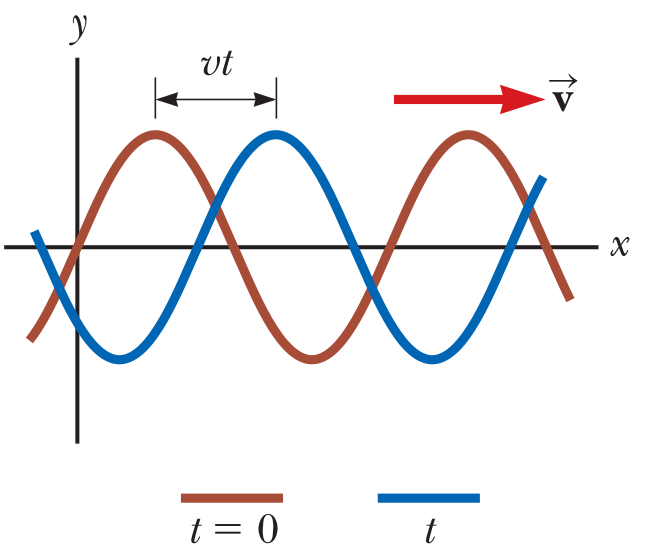
\includegraphics[width=\linewidth]{sin_wave.png}
  \caption{Onda sinusoidal que viaja hacia la derecha con una rapidez \(v\).}
  \label{fig:sin_wave}
\end{wrapfigure}
Para no complicar las cosas, continuemos con el ejemplo de la cuerda. Supongamos que la cuerda tiene un movimiento ondulatorio, y como ya hemos visto, la perturbación en la cuerda crea ondas transversales, y sinusoidales en este caso. 

La onda de color marrón de la figura \ref{fig:sin_wave} describe el estado inicial de la cuerda, es decir, es una instantánea de la onda sinusoidal en \(t=0\). Por otro lado la onda de color azul representa una instantánea de la misma cuerda en algún tiempo posterior \(t\), que llamaremos \(t_1\) para evitar confusión (aunque no se muestra en la figura).

Enfoquemos nuestra atención en un solo pulso de la onda. Si comparamos las instantáneas de la cuerda en \(t=0\) y \(t=t_1\), vemos que el pulso ha viajado una distancia \(v t_1\), donde \(v\) es la velocidad de propagación de la onda. 

Analizando el gráfico vemos que pueden ocurrir dos tipos de movimiento al mismo tiempo:
\begin{itemize}
  \item \textbf{El movimiento de la onda}: ya que la curva marrón, después de que transcurra el tiempo \(t\) llegará a la posición de la curva azul.
  \item \textbf{El movimiento de los elementos del medio}: se mueven de arriba a abajo con un \textit{movimiento armónico simple}. 
\end{itemize}

Si fijamos un tiempo determinado como \(t=0\), como el movimiento que describe la posición de los elementos del medio es un movimiento armónico simple, podemos describir la posición vertical de cada elemento del medio según su posición horizontal con la ecuación:
\[
  y(x, t=0) = A \sin(ax)
\]
donde \(A\) es la amplitud, \(a\), \(x\) es la posición horizontal y \(a\) es una constante a determinar. 

De la ecuación entonces, se ve que \(x=0\) se ve que \(y=0\), lo que coincide con la figura \ref{fig:sin_wave} en \(t=0\). El siguiente valor de \(x\) para el que \(y\) es cero es \(x=\lambda/2\) como se ve en la figura \ref{fig:sin_wave_2}

Por lo tanto, en base a estas observaciones, podemos escribir:
\[
  y(\lambda/2, t=0) = A \sin(a\lambda/2) = 0
\]
  
\begin{wrapfigure}{l}{0.35\textwidth}
  \centering
  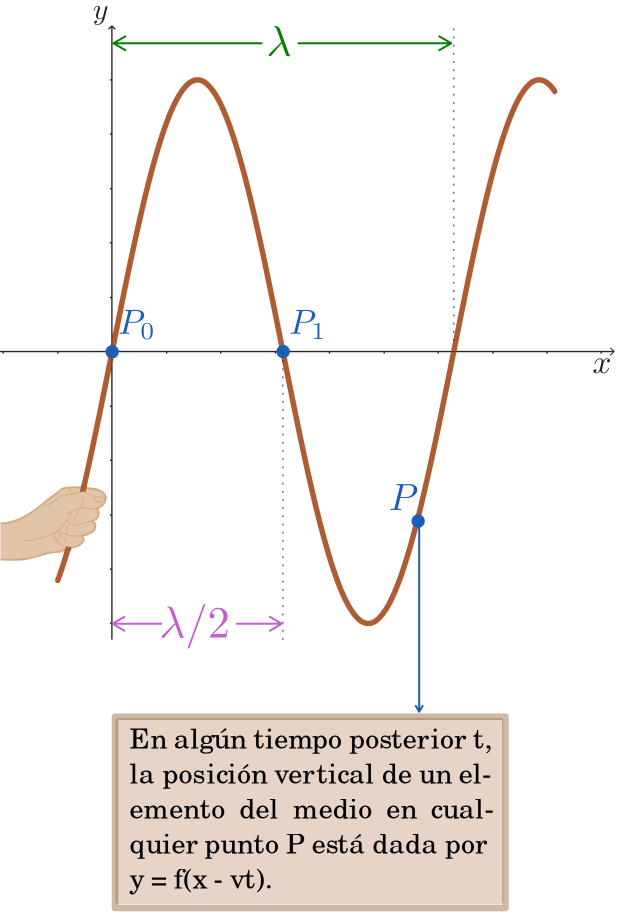
\includegraphics[width=\linewidth]{sin_wave_2.png}
  \caption{Instantánea de la cuerda en \(t=0\) donde una partícula \(P\) cualquiera tiene la misma posición vertical que \(P_0\) cuando la onda viaja una distancia \(v t\).}
  \label{fig:sin_wave_2}
\end{wrapfigure}
Para que esta ecuación sea cierta debe tener \(a\lambda/2 = \pi\) o \(a\lambda/2 = 2\pi\) (en base a la figura \ref{fig:sin_wave_2}), ya que estas posiciones están en fase. En consecuencia, la función que describe las posiciones de todos los elementos del medio a través del que viaja la onda sinusoidal para el instante \(t=0\) se puede escribir como:
\[
  y(x, t=0) = A \sin(\frac{2\pi}{\lambda} x) = 0
\]

Observe que la posición vertical de un elemento del medio es la misma simepre que \(x\) aumente un multiplo entero de \(\lambda\).

Como un pulso de la onda viaja a una velocidad constante \(v\), un elemento cualquiera \(P\) de la cuerda tendrá la misma posición vertical que \(P_0\) en el instante \(t_0\) cuando transcurra un tiempo \(t\) y el pulso de la onda viaje una distancia \(v t\). Entonces, en general podemos expresar la posición de cualquier elemento para todas las posiciones y tiempos como \(f(x - v t)\) donde \(f\) es una función periodica. En este caso \(f\) es la función seno, por lo que resulta:
\[
  y(x, t) = A \sin\left(\frac{2\pi}{\lambda} (x - v t)\right)
\]
  
Sabemos que \(v = \lambda / T ~~ \rightarrow ~~ T = \lambda/v\), por lo que si operamos la ecuación anterior obtenemos:
\begin{align*}
  y(x, t) & = A \sin\left[2\pi \left(\frac{x}{\lambda} - \frac{vt}{\lambda} \right)\right] \\
  y(x, t) & = A \sin\left[2\pi \left(\frac{x}{\lambda} - \frac{t}{T} \right)\right]
\end{align*}

Y recordando las cantidades básicas definidas en la sección \ref{sec:waves_basic_quantities}, podemos escribir:

\begin{equation}
  \boxed{y(x,t) = A \sin(kx - \omega t + \varphi)}
\end{equation}
donde \(\varphi\) es la fase inicial de la onda (en caso de que no comience en \(x=0\) como en el ejemplo).

\subsection{Energía asociada al movimiento ondulatorio}

La energía asociada al movimiento ondulatorio en ondas mecánicas proviene del hecho de que cada partícula del medio oscila en torno a su posición de equilibrio debido a la acción de una perturbación. Esta oscilación implica que hay energía almacenada en el medio, tanto en forma de energía cinética como potencial.

Vamos a continuar el análisis para una onda armónica transversal que se propaga en una cuerda (para continuar con el mismo ejemplo que venimos usando). 

\begin{tcolorbox}[myconclusion]
  Recuerda que un seno es la misma función que un coseno, pero desplazada \(\pi/2\).
\end{tcolorbox}

Consideramos una onda transversal que se propaga en la dirección \(x\), con desplazamiento en la dirección \(y\), y que \(\varphi = \pi/2\):
\[
y(x,t) = A \sin(kx - \omega t + \pi/2) = \boxed{A \cos(kx - \omega t)}
\]
donde:
\begin{itemize}
  \item \(A\) es la amplitud,
  \item \(\omega\) la frecuencia angular,
  \item \(k\) el número de onda.
\end{itemize}

Cada punto de la cuerda oscila verticalmente con esta función. En base a esta ecuación, podemos calcular la energía cinética y potencial de la cuerda.

\begin{tcolorbox}[myconclusion]
  Hemos supuesto una onda desplazada \(\pi/2\) para que la velocidad tenga signo positivo (ya que se obtiene al derivar la posición).
\end{tcolorbox}

\subsubsection{Energía cinética}

Una partícula de masa \(\mathrm{d}m\) en la cuerda tiene una velocidad vertical dada por su ecuación de M.A.S.:

\[
v_y(x,t) = \frac{\partial y}{\partial t} = -A \omega \sin(kx - \omega t)
\]

La energía cinética diferencial en un instante dado es:
\[
\mathrm{d}E_{\text{cin}} = \frac{1}{2} \, \mathrm{d}m \cdot v_y^2(x,t)
\]

Si la cuerda tiene densidad lineal \(\mu\) (en kg/m), entonces \(\mathrm{d}m = \mu \, \mathrm{d}x\). Por tanto:

\[
\mathrm{d}E_{\text{cin}} = \frac{1}{2} \mu \, A^2 \omega^2 \sin^2(kx - \omega t) \, \mathrm{d}x
\]

\subsubsection{Energía potencial}

La energía potencial elástica proviene de la deformación de la cuerda debido a su curvatura. En una cuerda ideal, se puede demostrar que, para pequeñas oscilaciones, la energía potencial tiene la misma forma media que la energía cinética. Se obtiene:

\[
\mathrm{d}E_{\text{pot}} = \frac{1}{2} \mu \, A^2 \omega^2 \cos^2(kx - \omega t) \, \mathrm{d}x
\]

\subsubsection{Energía total por unidad de longitud}

Sumando ambas contribuciones:

\[
\mathrm{d}E = \mathrm{d}E_{\text{cin}} + \mathrm{d}E_{\text{pot}} = \frac{1}{2} \mu A^2 \omega^2 \left[ \sin^2(kx - \omega t) + \cos^2(kx - \omega t) \right] \mathrm{d}x
\]

Como \(\sin^2 + \cos^2 = 1\), se obtiene la energía total por unidad de longitud:

\[
\frac{\mathrm{d}E}{\mathrm{d}x} = \mu A^2 \omega^2 \cdot \frac{1}{2}
\]


\subsubsection{Interpretación física}

La energía total transportada por la onda es proporcional al cuadrado de la amplitud \(A^2\), la densidad lineal \(\mu\) y al cuadrado de la frecuencia angular \(\omega^2\). Esta energía se transporta a lo largo de la dirección de propagación de la onda, sin que las partículas del medio se desplacen en esa dirección.

\subsubsection{Potencia transportada por la onda}

La potencia media (energía transportada por segundo) es:

\[
P = \frac{\mathrm{d}E}{\mathrm{d}t} = \frac{1}{2} \mu A^2 \omega^2 v
\]

donde \(v\) es la velocidad de propagación de la onda.
